\documentclass{article}
\usepackage{graphicx} % Required for inserting images
\usepackage{multicol}
\usepackage{cite}
\usepackage{amsmath}
\usepackage{amssymb}
\usepackage{subcaption}
\usepackage{hyperref}
\usepackage{ragged2e} 
\usepackage{caption}


\title{cnn}
\author{Murathan Sevinç}
\date{}

\begin{document}
\begin{figure}
\centering
  
\includegraphics[width=7cm]{ksbu.jpg}
\end{figure}
\title{Yapay Sinir Ağları,Derin Öğrenme Modelleri ve Uygulama Alanları}
\author{Murathan SEVİNÇ}

\maketitle 


\begin{center}
    \vfill
    \textbf{Bilgisayar Mühendisliği}\\
    \textbf{\date{Nisan 2024}}
\end{center}

\maketitle
%Giriş Sayfası 


\newpage
\section{Giriş}
\vspace{15pt}

 Derin öğrenme makine öğreniminin bir koludur. Makine öğreniminin başlarından günümüze kadar geçen
süreçte yapay zekaya olan ilgi giderek artmış ve günümüzde en çok kullanılan yapay zeka algoritmaları olan
derin öğrenme mimarilerinin ortaya çıkmasını sağlamıştır. Derin öğrenme mimarileri ile birlikte yapay zeka
problemlerinin çözümü için pek çok derin öğrenme yaklaşımları geliştirilmiştir. Endüstri, tıp, robotik, görüntü
işleme, bilgisayar görmesi, nesne tespiti, ses işleme-tanıma, çeviri, gelecek tahmini, finansal gibi pek çok
alanda akıllı çözümler üretmektedir. Bu çalışmada, derin öğrenme mimarileri ve algoritmaları incelenerek,
literatürde yapılmış çalışmalar ışığında uygulama alanları temelinde başarımları değerlendirilmiştir. Derin
öğrenme mimarileri ile birlikte derin öğrenmede kullanılan kütüphanelere yer verilmiştir. Bununla beraber
farklı problemlerin çözümlerine yönelik geliştirilen derin öğrenme mimarileri yer almaktadır. 

\vspace{10pt}
\textbf {Anahtar kelimeler:} Derin öğrenme, Yapay sinir ağları, Derin CNN, Konvolüsyonel sinir ağları


\begin{multicols}{2}
Günümüz mühendislik uygulamalarında insan
gibi düşünen, insan gibi davranışlar sergileyen
uygulamalara ağırlık verilmektedir. İnsan
olgusunun mühendislik uygulamalarında yer
alması için kullanılan adlandırma makine
öğrenmesi olarak bilinir (Goldberg ve Holland,
1988; Quinlan, 1986). İnsanın hayatı boyunca
öğrendiği şeylerin günlük yaşamda hayatını
kolaylaştırdığı ve deneyimlerine göre hareket
ettiğini örnek alarak aynı şekilde makine
öğrenmesi gerçekleştirilmeye çalışılmaktadır.
Makine öğrenmesinin özellikle sanayide üretim
kademesinde işlerin hızlandırılması, ürün
kalitesinin artırılması, ürünlerin sınıflandırılması
vb. gibi işlemleri hızlıca yapması için kullanımı
tercih edilmektedir (Sebastiani, 2002; Jordan ve
Mitchell, 2015). Bunun dışında güvenlik
uygulamalarında, sınıflandırma, medikal teşhis
ve tanı uygulamalarında, ileriye dönük tahminsel
yaklaşımlarda vb. (Michalski vd, 20013;
Sommer ve Paxson, 2010; Buczak ve Guven,
2016; Kourou vd, 2015; Holder vd., 2017) gibi
pek çok alanda kullanımı artmakta ve hayatı
kolaylaştırmaktadır. Bu gibi uygulamaların
gerçekleştirilmesi için kullanılan makine
öğrenmesindeki temel nokta insan beynindeki
nöronların çalışmasından faydalanılarak benzer
bir yaklaşımla makinanın öğrenmesini ve buna
göre davranmasını sağlamaktır (Fukushima,
1975). İnsan beynindeki sinir hücrelerinin
çalışma mantığından faydalanılarak yapay sinir
hücre modeli oluşturulmuştur (Harvey, 1994).
Bu yapay sinir hücre modeli zaman içerisinde
geliştirilmiş ve makine öğrenmesinde sıklıkla
kullanılmaya başlanmıştır. Günümüzde bu yapay
sinir hücre mantığı daha ileri seviyelere taşınarak
derin öğrenme mantıklı bir model kullanılmaya
başlanmıştır (Hinton vd., 2006). Yapay sinir ağı insan beyninin öğrenme
sürecinden etkilenerek ortaya atılmış bir
yaklaşımdır. 
\end{multicols}

\newpage
Bu yaklaşım ilk kez 1943 yılında
insan beynindeki hücrelerin yapısının
matematiksel modellemesi oluşturularak
gerçekleştirilmiştir (McCulloch ve Pitts, 1943). Burada temel amaç insan beyninin öğrenmesini
sağlayan sinir hücrelerinin matematiksel olarak
modellenerek bir bilgisayar sisteminin benzer bir
yaklaşım sergilemesini sağlamaktır. Bir insanın
öğrenmesi yan yana gelen sinapsların birbiriyle
olan bağlantılarıyla gerçekleşir (Hebb, 1949).
Sayısallaştırılmış bir sinir hücresi mantığı ile
yapay sinir ağları oluşturulmuştur.
Yapay sinir ağındaki matematiksel yaklaşımla
basit bir sinir ağı modellemesi yapılmış ve
bilgisayar sistemlerinde uygulanması
amaçlanmıştır. Sonraki yıllarda Hebb bu sinir
hücrelerinin tekrar eden durumlar karşılığında
öğrenmenin artığını belirlemiştir. Bu işlemde
nöronların matematiksel modellenmesi
nöronların gücünün artırılması gerektiğini ortaya
koymuştur (Hebb 1949).

\vspace{10pt}
\begin{figure}[h]
\centering
  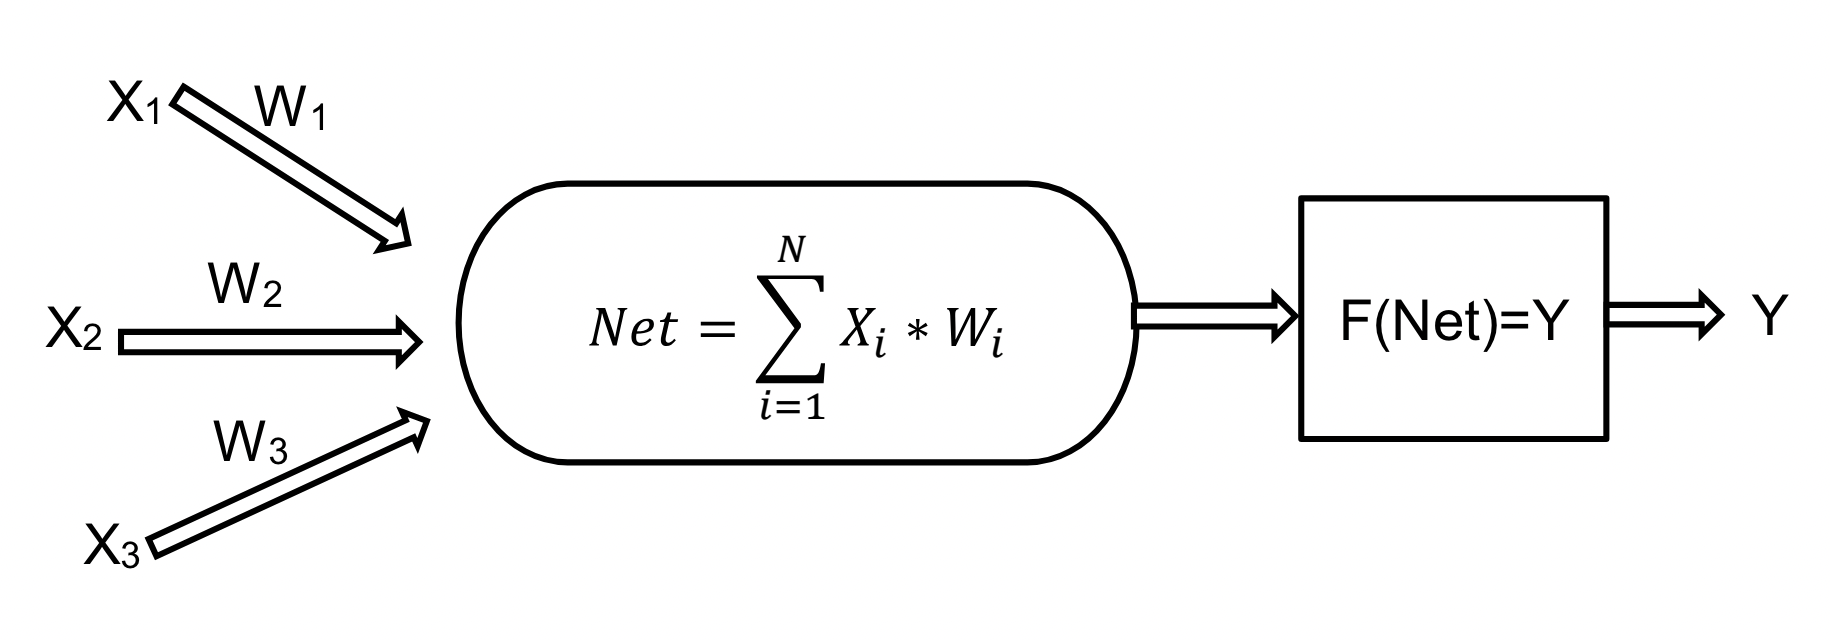
\includegraphics[width=10cm]{sema.png}
  \caption{Bir Sinir Hücresinin Matematiksel
Modelli \cite{ref1}}
(Perceptron Sinir Hücresi Modeli)
\end{figure}




\begin{multicols}{2}
Figure 1’de bir sinir hücresinin matematiksel
modeli gösterilmiştir. Burada X1, X2, X3 ile
belirtilen her bir dentriti göstermektedir.
Dendritlere ait ağırlıklar ise W1, W2, W3 ile
gösterilmektedir (Sarle, 1994). Her bir sinyalin
toplandığı Net ise çekirdeği temsil etmektedir.
Tüm sinyallerin ağırlıkları ile çarpılarak toplam
elde edilmektedir. Elde edilen Net toplam değeri
bir sonraki nörona belirli bir eşik değeri ile
gönderilmesi için F(Net) transfer fonksiyonu ile
gerçekleştirilmekte. F(Net) için kullanılabilecek
3 temel fonksiyon vardır. Keskin limitli transfer
fonksiyonun da giriş değeri 0’dan küçük içe çıkış
değeri 0’dır. Giriş değeri 0’dan büyük ise çıkış
değeri +1 değerini alır. Eşik değeri
fonksiyonunda ise girdi değeri toplamda 0 ve
daha küçük ise 0, 1 ve daha büyük girişler için 1,
0 ile 1 arasındaki değerlerde ise kendini alır.
Sigmoid fonksiyonu süreklilik gösteren ve türevi
alınabilen bir fonksiyondur. Doğrusal olmaması
sebebiyle sıklıkla tercih edilmektedir.Girdi değerine bağlı olarak 0-1 aralığında bir değer alır
(Stein, 1956)
\end{multicols}

\newpage
\begin{multicols}{2}
    1956 yılında Dartmaout’ta düzenlenen bir
konferansta zeka ile donatılmış bir bilgisayar
programını gerçekleştirme olanağını araştırmayı
öne sürmüşlerdir. Böylelikle yapay zeka terimi
kullanılmıştır. (J. McCarthy vd., 1956), LISP ile
yapılan satranç oyunu oynayan mantık teorisi
üzerine kurulu ilk yapay zeka programı
üretilmiştir. 1958 yılında Frank Rosenblatt
örüntü sınıflandırma için iki katmanlı perceptron
ağını önermiştir (Rosenblatt, 1958). Daha sonra
Robinson geliştirtiği yapay zeka algoritmasında
çözünürlük ilkesine dayanan makine odaklı bir
mantık makalesini yayınlamıştır (Robinson,
1965). 1970’li yılların ortalarına kadar yapay
sinir ağlarının karanlık döneme girip durma
noktasına gelmiştir. Bu dönemde XOR
probleminin çözülememiş olması yapay zekanın
geleceği konusunda ciddi kaygılara yol açmıştır.Ve yapay zeka bu noktadan sonra duraklama
dönemine girmiştir (Minsky, 1969). 1970 ve
1980’li yıllar arasında bilgiye dayalı sistemler
ağırlıkla yer almıştır. 1970’lerin ortalarında XOR
probleminin çözümü üzerine yaklaşım
getirmiştir (Werbos, 1974). Hopfield neuro
biyolojik yapıların makinalar içinde
uygulanabilirliği konusunda yayınladığı bir
makale ile makine öğrenimine dikkat çekmiştir
(Hopfield, 1982). 1986 yılında yayınlanan bir
kitapta paralel dağıtık sistemlere ait problemlerin
çözümleri ortaya konmuştur. Burada XOR
probleminin çözümü de yer almaktadır
(McClelland, 1986). Aynı yıl Fukushima yaptığı
çalışma ile örüntü tanıma için bir yaklaşım
getirmiştir (Fukushima, 1986). Daha sonra
Broomhead ve Lowe yaptıkları çalışma ile radial
tabanlı sistemleri çok katmanlı sistemlere
alternative olarak geliştirmişlerdir (Broomhead ve Lowe, 1988). Probalistik ağlar (Specht 1988)
ve genel regrasyon ağları (Specht, 1991) ortaya
konmuştur. Yapılan çalışmalarla yapay zeka,
yeniden yön bulmuştur. Pek çok bilimsel
çalışmalarda kullanılır hale gelmiştir (Yadav,
2015).
\vspace{10pt}

Yapay sinir ağı modeli teorisiyle birlikte makine öğrenmesi konusunda bir çağ başlatılmıştır.İnsan düşüncelerine göre karar verme yetisi
yapay sinir ağı modeli ile makinelere de
geçmiştir. Lineer denklemlerin çözümünde
başarılı sonuçlar elde edilmiştir (Sajikumar ve
Thandaveswara, 1999). Literatüre bu yöntemle
kazandırılmış pek çok yaklaşım yer almaktadır.
Yapılan çalışmalarda ileri beslemeli yapay sinir
ağı modeli kullanılmış ve başarım oranı belirli bir
sınırda kalmıştır (Morris ve Rubin, 1991). 
\vspace{10pt}

İlk yapılan yapay sinir ağı modelinde tek
katmanlı ileri beslemeli yapay sinir ağı modeli
kullanılmıştır (Lippmann, 1987).Elde edilen
sonuçlar belirli bir oranda kalmış ve üzerine
çıkamamıştır.Daha sonrasında yapılan
çalışmalarda geri beslemeli sinir ağı modeli
oluşturulmuştur. Geri beslemeli sinir ağı modeli
ile elde edilen sonuçlar üzerinde düzenlemeler
yapılarak daha başarılı sonuçlara ulaşılmıştır.
Yapay sinir ağı modelleri ile yapılan çalışmalar
artarken halen lineer denklemlerde sağlıklı
çalışan bu sistem lineer olmayan sistemlerde
çalışmamakta ve doğru sonuçlar
üretilememekteydi (Jain vd., 1996). 
\end{multicols}

\newpage

    Linear olmayan problemlerin çözüme ulaşması
çok katmanlı yapay sinir ağı modeli ortaya
çıkarmış ve geri beslemeli çok katmanlı sinir ağı
modeli ile lineer olmayan denklemler çözüme
kavuşmuş. Ve sinir ağlarına olan ilgi yeniden
artmıştı (Eberhart ve Kennedy, 1995).
Çok katmanlı sinir ağı modelinin ortaya
çıkmasıyla birlikte katman sayısının artırılarak
daha iyi sonuçlar vermesi için Convulotional
Neural Network (CNN) geliştirilmiştir. Burada
yer alan sinir ağı modelinde gizli katmanlar yer
almakta ve elde edilen sonuçlar oldukça başarılı
olmaktadır (Pan vd., 2000). Konvolüsyonel sinir ağlarının gelişmesi ile birlikte sınıflandırma işlemleri daha başarılı
sonuçlar vermiştir. Konvolüsyon işlemi ile obje
üzerindeki hatlar belirli hale getiriliyor ve sinir
ağı modeli içine dahil ediliyordu (LeCun ve Bengio, 1995). 2006 yılında Geoffrey Hinton ve Ruslan Salakhutdinas tarafından yayınlanan makale ile derin öğrenme terimi ortaya atılmış ve
derin öğrenme çalışmaları başlamıştır (Hinton ve Salakhutdinas, 2006). Sinir ağlarının gelişim süreci tablo 1’ de verilmektedir.


\vspace{15pt}

{\centering \textbf{Tablo1. Sinir ağlarının tarihsel dönüm noktaları}}
\vspace{10pt}

\begin{tabular}{c|p{5cm}|p{5cm}}
  
  \textbf{Yıllar} & \textbf{Gerçekleşen} & \textbf{Yayıncı}\\
  \hline
  1940 & Elektronik Beyin (1943) & S. McCulloch, W. Pitts \\
  \hline
  1950 & Perceptron – Tek katmanlı algılayıcı (1957) & M. Hoff, B. Widrow,  F. Rosenblatt \\
  \hline
  1960 & Multi Layer Perceptron- Çok katmanlı algılayıcı (1965) & A.G. Ivakhnenko, V.G. Lapa \\
  \hline
  1970 & Neocognitron (1979) & K. Fukushima \\
  \hline
  1980 & Backpropagation (1986) & D.Rumelhart,
  
  G.Hinton, R.Williams \\
  \hline
  1990 & XOR prolemleminin ortaya çıkışı  Destek Vektör Makineleri (SVM-Support Vector Machine) & S. Hochrelter
Schölkopf, Burges, Vapnik \\
  \hline
 2000 & - & - \\
  \hline
  2010 & Deep Nural Networks – Derin Sinir ağları (2006) & G. Hinton \\
  \hline
\end{tabular}
\vspace{10pt}
\section{Derin Öğrenme Materyal ve Yöntemleri}
\vspace{10pt}


Hinton’un yapmış olduğu çalışmalarla
yayınlamış olduğu makalede yapay sinir ağlarına
yeni bir yaklaşım getirmiştir. Bu yaklaşım derin
öğrenme (Deep Convolution Neural Network)
olarak adlandırılmıştır (Hinton vd., 2006).
Konvolüsyonel sinir ağları çok katmanlı sinir
ağları olarak bilinmektedir. Bu sinir ağı
sistemiyle önemli çalışmalar yapılmış ve
başarımı yüksek sonuçlar elde edilmiştir. Derin
konvolüsyonel sinir ağı elde edilen bu
başarımları daha yüksek seviyelere çıkararak
önemli bir başarıya imza atmıştır (Krizhevsky
vd., 2012; LeCun vd., 1998; Szegedy vd., 2015;
Zeiler ve Fergus, 2013; Szegedy vd., 2015). 

\newpage

Konvolüsyonel sinir ağı ile sinyal işleme, video
analizi, görüntü analizi ve tespiti, sınıflandırma,
medikal görüntü işleme gibi pek çok alanda
önemli işler çıkarmıştır. Bu sinir ağı kullanılırken
bazı aşamalar gerçekleştirilmektedir. Bunlar ön
işlem, özellik çıkarımı ve sınıflandırma-tespit
şekilde tanımlanmaktadır. Her bir aşamasında
özel yaklaşımlar sergilenmekte ve doğruluğu
artırmaya yönelik çalışmalar yapılmaktadır.
Özellikle özellik çıkarım işlemi için pek çok
farklı yaklaşım sunulmuştur. Özellik çıkarımı ile
tespit edilmesi istenen olaya ait belirgin noktalar ortaya çıkarılmaya çalışılmaktadır. Sonraki
süreçte ise yapay sinir ağları kullanılarak
belirlenen özelliklere ait sınıfın tespiti için sinir
ağları kullanılmaktadır (Snoek vd., 2005; Li vd.,
2010; Scherer vd., 2010).
\vspace{10pt}

Derin öğrenme ile daha önce yapılan pek çok
işlem bir arada yürütülerek sonuca gidilmektedir.
Burada özellikle ön işlem ve özellik çıkarımı gibi
yapılar göz ardı edilmekte ve sinir ağı içerisinde
bu işlemler otomatik olarak yapılmaktadır. Derin
konvolüsyonel sinir ağında özellik çıkarımı ağın
içerisinde belirlenmekte ve katmanlar içerisinde
tespit edilmesi istenen yapıya ait özellikler
belirlenmektedir. Alt katman ile üst katman
arasında bağlantılı hiyerarşik bir yapı
bulunmaktadır. Özellik çıkarımı için özel bir
safha bulunmamaktadır. Katmanlar içerisindeki
yapısında nesne-olaya ait belirgin özellikler
belirlenmekte (Hinton ve Salakhutdivot, 2006)
ve sonraki katmana aktarılmaktadır (Bengio,
2009). Şekil 2’ de yer alan görüntüde uydu
görüntülerini sınıflandırılmasını sağlayan
konvolüsyonel sinir ağı modeli yer almaktadır
(Doğan ve Türkoğlu, 2017). 

\vspace{10pt}
\begin{multicols}{2}
Yapay sinir ağlarında sınıflandırma yapılırken
kullanılan 3 temel öğrenme yapısı vardır bunlar
öğretmenli öğrenme (Supervized) (Shipp vd.,
2002), öğretmensiz öğrenme (Unsupervized)
(Hastie, 2009) ve takviyeli öğrenmedir
(Reinforcement) (Chapelle, 2006).

Öğretmenli öğrenmede yapay sinir ağına giriş
verisi olan y(t) verisi, çıkışta d(t) olarak çıkacağı
bilgisi verilmiştir. Oluşturulan sinir ağı içerisinde
sonuca ulaşmak için ağırlıklar belirlenir. Bu
ağırlıklara göre y(t) girdi verisinin d(t) çıkış
sonucunu elde edilmesi için verilen örneklere
göre ağırlıklar güncellenir. Ağırlıkların
güncellenmesi işlemi belirlenen iterasyon sayısı
kadar devam ederek öğrenme işlemi gerçekleşir
(Shipp vd., 2002). 

Öğretmensiz öğrenmede ise bir çıkış bilgisi
verilmeksizin giriş görüntüleri ağın girişine
uygulanır. Ağdaki katmanlarda sonuç verisi
oluşturulur. Buna göre oluşan çıkışlarda benzer
değerlere sahip olan sonuçlar bir kümeye alınır.
Oluşan her bir küme bir sınıfı temsil eder (Hastie,
2009). 

Takviyeli öğrenmede ise ağa giren verinin çıkış
verisi ne olması gerektiği konusunda bir bilgi
verilmez. Girdi verisinin çıkışı üretilmesi
beklenir. Bir öğretmen yardımıyla üretilen çıkışa
göre sonucun doğru ya da yanlış olduğu bilgisi
verilir. Girdi verisi yanlış sonucu ürettiğinde ağın
ağırlıklarının doğru sonucu üretmesi için tekrar
güncelleme yapar (Chapelle, 2006).
\end{multicols}

\newpage
\begin{multicols}{2}
    

\subsection{Konvolüsyonel Sinir Ağları (Convulational Neural Network)}
Çok katmanlı ileri beslemeli bir yapay sinir ağı
olan konvolüsyonel sinir ağı (CNN) özellikle
görüntü analizlerinin yapılması için
kullanılmaktadır. Hayvan görü sistemine
dayanan bir yaklaşımla ortaya atılmıştır (Hubel
ve Wiesel, 1968). Filtrelemeye dayalı bir
yapıdadır. Kullanılacak olan fitre ile görüntünün
özelliğini belirtecek öznitelikleri belirgin hale
getirir. Özellikle sınıflandırıcı işlemlerinde
başarılı sonuçlar üretmektedir. Filtreler farklı
boyut ve değerlerde kullanılarak baskınlık düzeyi
az olan özniteliklerin ortaya çıkmasını sağlar
(Fukushima, 1982; Simard, 2003). Şekil 2’de
konvolüsyonel sinir ağına ait örnek bir mimari
görülmektedir.

İlk olarak LeCun ve arkadaşları tarafından
gradyan temelli bir yaklaşım sunularak ortaya
çıkan ağ yapısına konvolüsyonel sinir ağı adı
verilmiştir. Oluşturulan bu yapay sinir ağına ise
LeNet adı verilmiştir (LeCun vd., 1998).
Çok katmanlı bu sinir ağı içerisinde birden fazla
konvolüsyon katmanı, tam bağlı katman,
aktivasyon katmanı, sınıflandırıcı katman,
havuzlama katmanı ve bunlara ek katmanlar yer
almaktadır. Her katman kendi işlevini yürüterek
sınıflandırıcı katmanda sonuç üretilmektedir.
Derin öğrenme yapıları içerisinde en çok
kullanılan sinir ağı konvolüsyonel sinir ağlarıdır.
Daha çok sınıflandırma ve tespit işlemleri için
kullanılmaktadır. Sinir ağı içerisindeki
katmanlarla sınıflandırılacak öğelere ait
öznitelikler belirlenerek sınıflandırıcı katmanı ile
öğeler sınıflandırılır.

\subsection{Tekrarlayan Sinir Ağı (Recurent Neural Network)}
Elman tarafından tasarlanan basit tekrarlayan
sinir ağları (Simple Recurrent Network-SRN) dil
bilimciler ve psikanaliz için çığır açan bir
yaklaşım olmuştu. Elmanın yayınladığı
makalede konuşma akışı üzerindeki gizli yapı
üzerinde çalışılan bir öğrenme sürecini temsil
ediyordu. Örüntü kümelemesinde fiil ve isim
kategorizasyonu açık şekilde birbirinden
ayrılıyordu. Ayrıca canlı-cansız, insan-hayvan,
avcı-yırtıcı gibi kategorilerde ayrılmıştı. (Elman,
1990). 

Tekrarlayan sinir ağıları(RNN), sadece ağa giren
giriş örneklerini değil daha önce zaman serisi
içerisindeki giriş örneklerini de alırlar. Bu sinir
ağının amacı ardıl şekilde gelen verilerin
kullanılmasıdır. Geleneksel sinir ağlarında
girişler birbirlerinden bağımsız olarak ağa giriş
yapar. 

Ya da kurulacak bir cümlede art arda gelen
kelimelerin akabinde cümlenin devamının nasıl
geleceğini gösteren kelimenin tahmin edilmesi
işlemi örnek olarak verilebilir. İki tür RNN vardır
bunlar; İki yönlü RNN’ler (Bidirectional RNNs)
(Schuster ve Paliwal, 1997) ve Derin RNN’lerdir
(Deep RNNs) (Schmidhuber, 1992).
\vspace{10pt}


\begin{minipage}{\linewidth}
    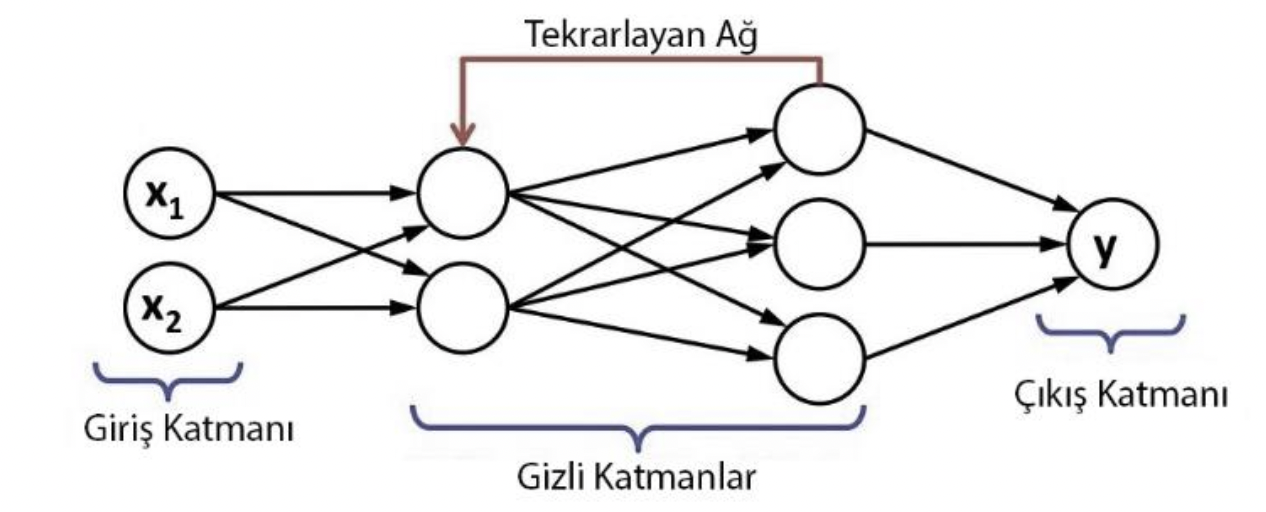
\includegraphics[width=1\linewidth]{tekrarla.png} 
    \label{fig:Şekil tekrar}
\end{minipage}

\centering {Tekrarlayan sinir ağı modeli \cite{ref2}}

\end{multicols}

\newpage
\begin{multicols}{2}
\subsection{Uzun-KısaSüreli Hafıza (LSTM- Long
Short-Term Memory)}

RNN mimarilerinde zaman dizeleri aralarında
bağlam boşlukları olması halinde sonraki dizenin
tahmin edilmesi çok zor bir durumdur (Bengio
vd, 1994). Bu durum RNN’ler için oldukça
dezavantajlı bir durumdur. Hochreiter ve
Schmidhuber yapmış oldukları çalışmada bu
durumu ortadan kaldıracak uzun ve kısa süreli hafıza LSTM öne sürmüşlerdir (Hochreiter ve
Schmidhuber, 1997).

LSTM ağlarının RNN ağlarından bir farkı
yoktur. Fakat gizli durumu hesaplamak için
LSTM ağlarında bir yapı kullanılır. LSTM
içerisinde hafıza hücreleri yer alır. Önceki
durumu ve girdi bilgisini tutan bir hücredir. Ağ
mimarisi içerisinde yer alan bu hücreler hangi
verinin tutulacağına ya da hangi verinin
sileceğine karar verirler. Sonraki aşamada ise
önceki durumu mevcut bellek ile giriş verisini
birleştirirler. Böyle bir yaklaşımla uzun vadeli
bağımlılıkların ortadan kaldırılarak veri
dizilerinin devam ettirilmesi mümkün kılınır.

\vspace{5pt}
\begin{minipage}{\linewidth}
    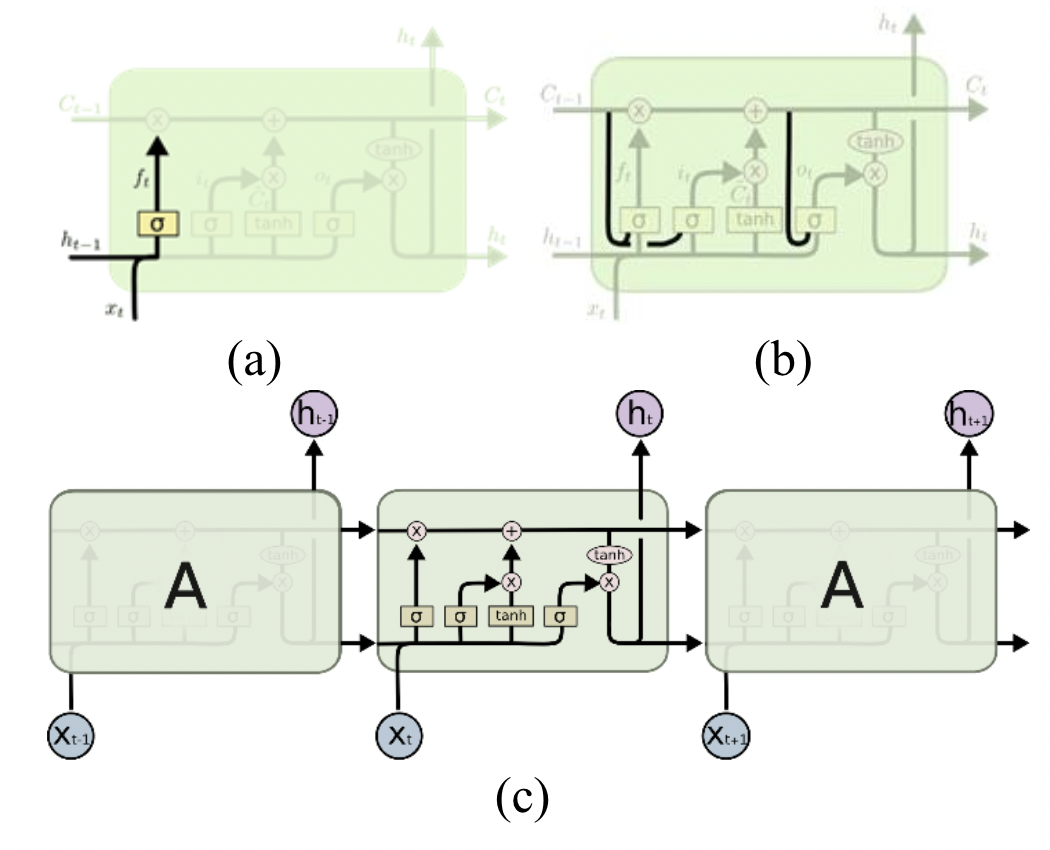
\includegraphics[width=0.8\linewidth]{unutmakatmani.png} 
    \label{fig:Şekil 6}
\end{minipage}

\vspace{10pt}
    Şekilde LSTM bloğu yer almaktadır. Burada
yer alan gözetleme ve unutma kapısında unutma
kapısı durumu sıfırlamak, gözetleme kapısı
bağlantıları öğrenmeyi kolaylaştırmak için
kullanılmaktadır (Gers vd., 1999; Gers ve
Schmidhuber, 2000). 

\subsection{KısıtlıBoltzmann Makinesi (RBMRestricted Boltzmann Machine)}

1987 yılında Hinton, Sejnowski ve Ackley
tarafından yayınlanan makale ile öğrenme
algoritmalarının prensipleri anlatılmıştır. Simetri
prensibiyle hücreler arası bağlantılarla
yenilemeli kısıtları yapmanın Bolzmann Makinesi ile olabileceğini ortaya atmışlardır
(Ackley vd., 1987). 

1993 yılında Kappen yayınladığı “Olasılık
Tahmininde Boltzmann Makinelerini
Kullanmak: Sinir Ağı Öğrenimi için Genel Bir
Yapı” başlıklı makalesinde, Boltzmann
Perceptron modeli ile bir uygulama yapmıştır. Bu
uygulamada bileşik olasılıksal dağılımları
tahmin edebileceğini belirtmiştir (Kappen,
1994). 

Her bir düğüm bir nörondur. Ve hesaplamalar bu
düğümlerde yapılır. Her düğüm gizli katmanda
yer alan bir başka düğümler (nöron) ile bağlanır.
Aynı katmandaki düğümler birbirleriyle
bağlanmazlar. Yani katmanlar arası iletişim
yoktur. Bu yüzden kısıtlı boltzman makineleri
olarak adlandırılır. Görünür katmanda girdiler
hesaplanır ve bir sonraki düğüme o girdiyi iletilip
iletilmeyeceği rastgele olarak belirlenir (Hinton,
2012). 

\vspace{10pt}
\begin{minipage}{\linewidth}
    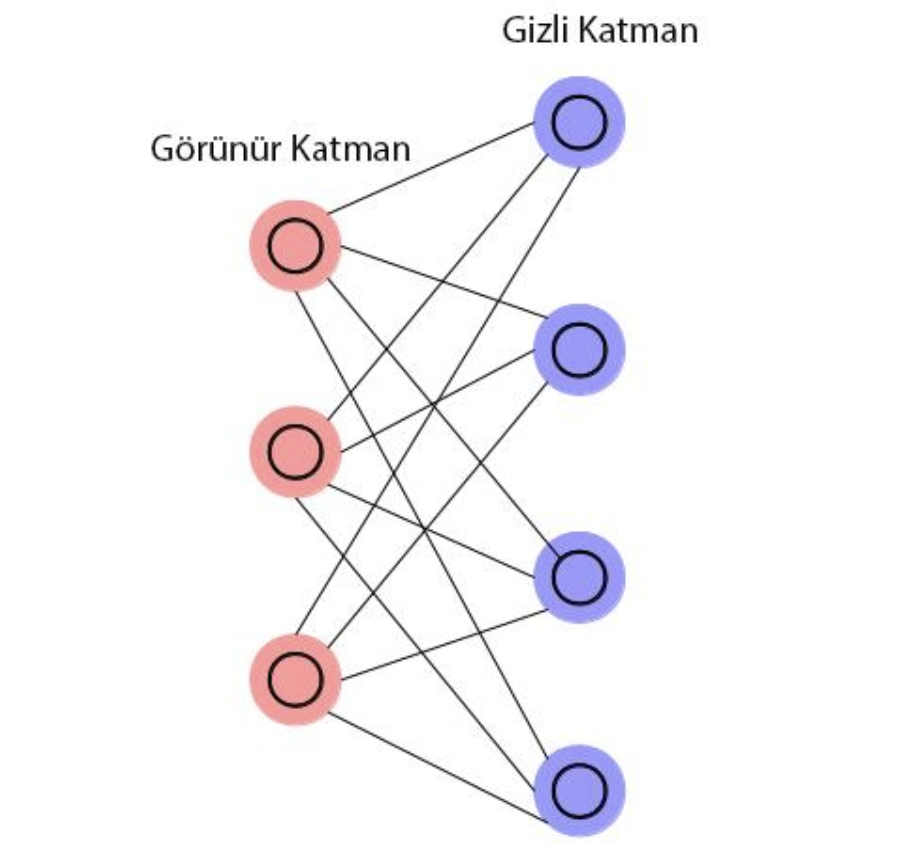
\includegraphics[width=0.8\linewidth]{gorunurkat.png} 
    \label{fig:Şekil 7}
\end{minipage}
\begin{center}
    Kısıtlı Boltzman Makinesi \cite{ref3}
\end{center}
\end{multicols}

\newpage
\begin{multicols}{2}
\subsection{Derin İnanç Ağı (DBN-Deep
Belief Network)}

Hinton RBM’i kullanarak Derin İnanç Ağları
(DBN) yığınını oluşturmuş ve bu ağın eğitilip
eğitilebileceğini göstermiştir. Derin inanç ağları
veri setinin hiyerarşik temsilini çıkarmayı
amaçlayan grafiksel modellerdir. Örnek bir
makine yapısı, şekil 8’de gösterilmiştir. Şekilde
görünür giriş katmanını h ise gizli katmanı temsil
eder. Art arda eklenen kısıtlı boltzman
makineleri katmanlarından oluşan bir sinir ağı
yaklaşımıdır. Kısıtlı boltzman makinelerinin
sırasıyla eğitilerek öğrenilmesiyle gerçekleşir.
Giriş uygulanan veri ile gizli katman arasında
olasılıksal bir dağılım modellenir (Hinton, 2006).

\begin{minipage}{\linewidth}
    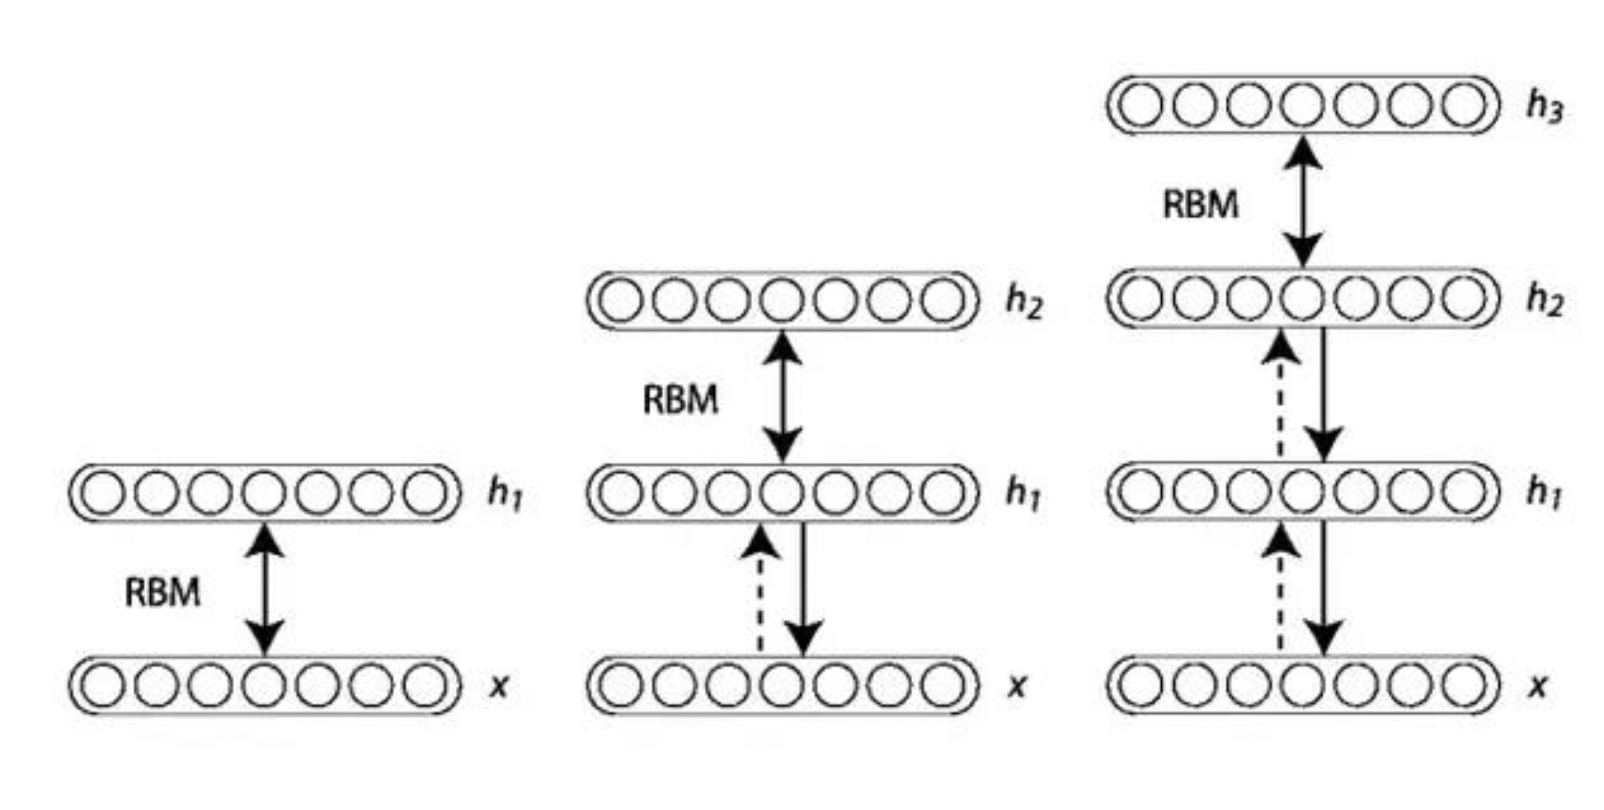
\includegraphics[width=0.8\linewidth]{kisitlibol.png} 
    \label{fig:Şekil 8}
\end{minipage}
\begin{center}
    Ard arda gelen kısıtlı boltzman
makineleri örneği \cite{ref4}
\end{center}

\vspace{5pt}
Grafiksel model katmanından oluşan hem
yönlendirilmiş hem de yönsüz kenarlı bir sinir
ağı sınıfıdır (Boureau, 2008). Örüntü tanıma ve
üretme konularında etkindir (Huang vd., 2007;
Bengio vd., 2007). Denetimsiz ön tanımlı bir
sinir ağıdır. Derin inanç ağı modeli örneği şekil
9’da görülmektedir.
\vspace{10pt}

\begin{minipage}{\linewidth}
    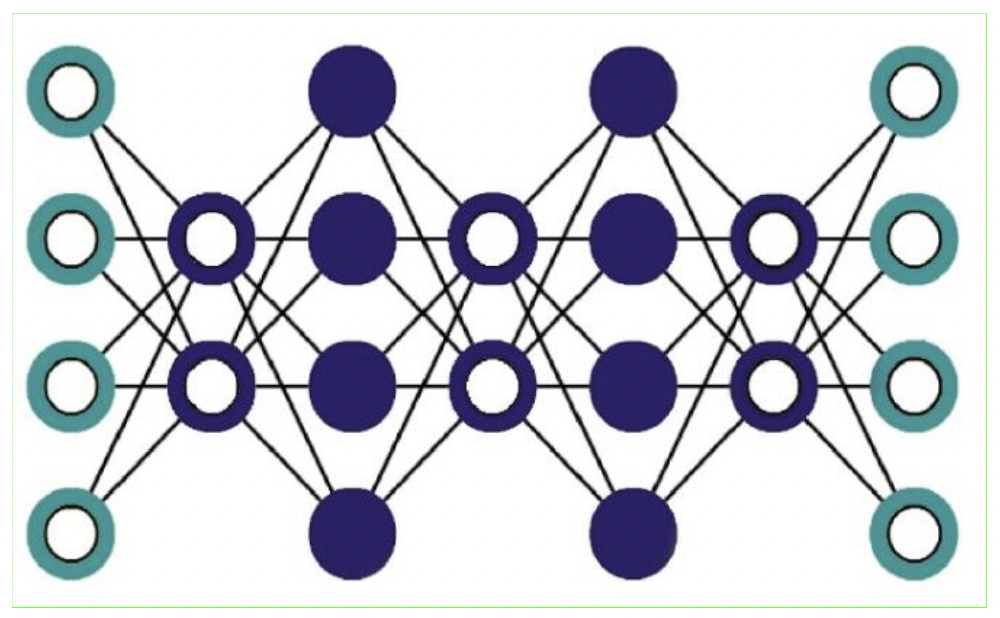
\includegraphics[width=0.8\linewidth]{inancagi.png} 
    \label{fig:Şekil 9}
\end{minipage}
\begin{center}
    Derin inanç ağı modeli \cite{ref5}
\end{center}


\subsection{Derin Oto-kodlayıcılar (Auto Encoder)}
Yapay sinir ağı modellerinden biri olan derin oto
kodlayıcılar denetimsiz öğrenme tabanlı makine
öğrenme sistemidir. Bu sinir ağı diablo ağı
olarakta adlandırılmaktadır (Bengio, 2009; Lu,
2013). Yıllarca sinir ağlarının temel bir parçası
olmuştur (Hinton ve Zemel, 1994). Derin
öğrenme mimarilerinin ortaya çıkmasıyla
beraber derin öğrenme mimarileri içerisinde yer
almaya başlamıştır (Baldi, 2012). Oto
kodlayıcılar giriş veri kümesini sıkıştırarak en az
kayıpla en iyi öğrenmeyi amaçlar. İleri beslemeli
bir sinir ağıdır (Krizhevsky ve Hinton, 2011).

Temel olarak 3 katmandan oluşmaktadır. Girdi
katmanı, gizli katman ve çıktı katmanı. Giriş ve
çıkış katmanındaki nöron sayıları eşit olmakla
birlikte gizli katmandaki nöron sayısı
değişkenlik göstermektedir. Şekil 10’de bu
durum gösteren oto kodlayıcı görülmektedir.
Gizli katman içerisindeki nöronların sayısı giriş
ve çıkış katmanında yer alan nöronlardan daha az
olduğunda veri kümesi sıkıştırılır. Böylelikle
daha az veri ağ içerisinde yer alır. Bu da ağın
performansında etkili olmaktadır (Vincent vd.,
2010; Vincent vd., 2008). 

\vspace{20pt}
\begin{minipage}{\linewidth}
    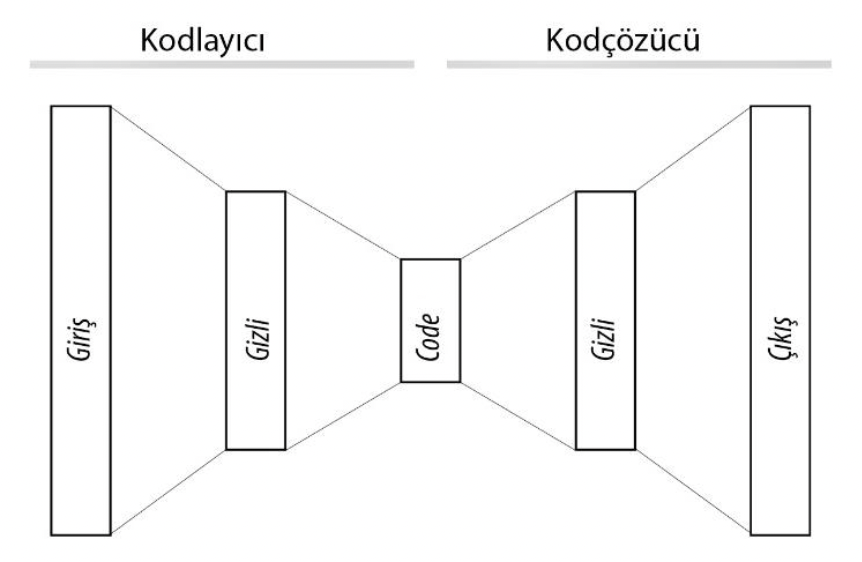
\includegraphics[width=0.8\linewidth]{encode.png} 
    \label{fig:Şekil 8}
\end{minipage}
\begin{center}
    Oto Kodlayıcı şeması \cite{ref6}
\end{center}
\end{multicols}

\newpage
\section{Derin Öğrenme Katmanları}


\begin{itemize}
    \item Giriş (Input) Katmanı
    \item Konvolüsyon(Convolution) katmanı
    \item Aktivasyon (Relu) katmanı
    \item Havuzlama (Pooling) Katmanı
    \item Tam Bağlı (Full-Connected) Katman
    \item Dropout Katmanı
    \item Sınıflandırma (Classification) katmanı
    \item Yumuşatma (Softmax) Katmanı
    \item Normalizasyon (Normalization) Katmanı
\end{itemize}

\begin{figure}[h]
\centering
  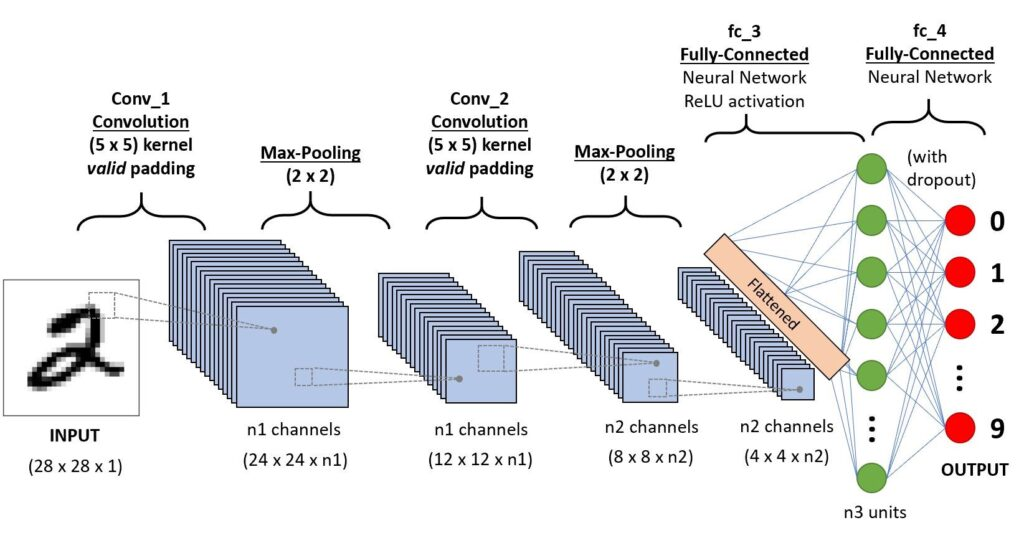
\includegraphics[width=13cm]{net.jpeg}
  \caption{Derin Öğrenme Katmanları \cite{ref7}}
\end{figure}
\vspace{15pt}

\newpage
\section{Derin Öğrenme Algoritmaları}
\vspace{5pt}
\begin{itemize}
    \item LeNet
    \item AlexNet
    \item ZF Net
    \item VggNet
    \item GoogleNet
    \item ResNet
\end{itemize}

\begin{center}
    
\textbf{Tablo 2.Derin öğrenme algoritmaları}
\end{center}
\vspace{10pt}

\begin{tabular}{c|p{3cm}|p{3cm}|p{2cm}|p{3cm}}
  \textbf{Yıl} & \textbf{Derin Öğrenme Algoritması} & \textbf{Geliştirici} & \textbf{Hata Oranı} & \textbf{Parametre Sayısı} \\
  \hline
  1998 & LeNet & Yann LeCun ve Arkadaşları &  & 60Bin\\
  \hline
  2012 & AlexNet & Alex Krizhevsky,Geoffrey Hinton & \%15.3  & 60Milyon\\
  \hline
  2013 & ZFNet & Matthew Zeiler ve Rob Fergus & \%14.8 & \\
  \hline
  2014 & GoogleNet & Google & \%6.67 & 4Milyon\\
  \hline
  2014 & VGGNet & Simonyan, Zisserman & \%7.3 & 138Milyon\\
  \hline
  2015 & ResNet & Kaiming He & \%3.6 & \\
\end{tabular}
\vspace{10pt}
\section{Derin Öğrenme Kütüphaneleri}

\begin{multicols}{2}
\begin{itemize}
    \item Tensorfflow
    \item Caffe
    \item Theano
    \item Torch
    \item DeepLearning4j
    \item Keras
    \item Lasagne
    \item Cognitive Network Toolkit (CNTK)
    \item DIGIT
    \item Pylearn2
    \item MXNET    
\end{itemize}
\end{multicols}

\newpage
\section{Derin Öğrenmenin Uygulama Alanları}
\vspace{10pt}
\begin{itemize}
\item Bilgisayar Görmesi (Computer Vision)
\item Sınıflandırma (Classification)
\item Nesne Tespiti (Object Detection)
\item Ses (Audi-Wave-Speech)
\item Medikal (Medical)
\item Endüstri (Industrial)
\end{itemize}

\section{Sonuçlar ve Tartışma}
\begin{multicols}{2}
Yapay zeka mimarileri geçmişten günümüze
gelindiğinde pek çok alanlarda kullanılmaktadır.
Yapay zeka yaklaşımlarının tarihsel gelişimi
makine öğrenmesinin ne denli bir hızla
geliştiğini göstermektedir. Elektronik ve
bilgisayar sistemlerinin hemen hepsinde kontrol,
denetim, tahmin, modifikasyon, üretim, eğlence
amaçlı bir yaklaşımı görmek mümkün. Caddede
bilbordlarda, oyun salonlarında, araba, uçakta,
dinlediğimiz bir müzikte, izlediğimiz bir filmde,
televizyonlarda pek çok uygulamada, hava
tahminlerinde, hastanede, güvenlik
sistemlerinde, savunma sanayisinde, finansal sektörlerde ve pek çok günlük yaşam aktivasyonlarında görmek mümkündür. 

Derin öğrenme sistemlerinin bu kadar geliştiği
bir ortamda şirketler, devletler, kurumlar arge
için bu konuya ciddi şekilde eğilim
göstermişlerdir. Pek çok büyük bilişim şirketi bu
konuda atılımlar yapmış yeni yaklaşımlar
getirmiştir. Konunun gelişimine göre yeni
uygulamalar ve bakış açıkları geliştirmişlerdir.
Google, Microsoft, Baidu, IBM, Apple, Nvidia,
Facebook, Twitter, Amazon ve daha birçok şirket
derin öğrenmeyle ilgili çalışmalar yapmıştır. 

Yapılan çalışmalara bakıldığında derin öğrenme
mimarileri yapay zeka teknolojilerine yeni bir
yaklaşım getirdiği ve çığır açtığı görülmektedir.
Derin öğrenme mimarilerinin gelecek
tahminlerine yönelik çalışmaları günümüz
teknolojilerini birkaç yıl ileri taşıdığı
düşünülmektedir. İnsan hayatını kolaylaştırmak,
sağlıklı bir yaşam sürdürebilmek için derin
öğrenme mimarilerinin çok etkin şekilde
hayatımızda yer almaya başladığı görülmektedir.

Gelecekte günlük yaşamın her noktasında yer
alacak olan bu mimarilerin otomot bir dünyanın
kapısını aralayacağı düşünülmektedir. Kendi
kendine gideceği yere varan araçlar, daha güvenli
yollar, insansız hava ve kara araçları, taşıma
alanında bir başkalaşıma doğru götürecek
çalışmalar yapılmaktadır.

\newpage 
 Tıp alanında; hastalık
tanı ve teşhisin daha hızlı gerçekleşebileceği,
doktorun yapmış olduğu ameliyatların bir
kısmını robotların yapabileceği, kendi kendine
hastaya cevap verebilecek sistemlerin
oluşturulabileceği, hastanın sağlık merkezlerine
uğramadan tanı-teşhis konabileceği sistemler
üzerine çalışmalar yapılmaktadır. Robotik sistemlerde farklı bir noktaya getirecek
ve robotların insan yaşamında etkin bir rol
oynayacağı bir dünya için pek çok çalışma
yapılmaktadır. Pek çok özel şirket insan gücünün
yerini robotik sistemlere bırakacağı öncü
çalışmalar yapmaktadır. Tarımsal alanlarda
sulama, bakım, gübreleme, toprak analizlerinin otomatik yapılacağı ulusal sistemler için derin
öğrenme tabanlı çalışmalar devam etmektedir.
Savunma sanayinde kullanılan pek çok yapay
zeka teknolojisi bulunmaktadır.
Günümüzde pek
çok savunma araçları derin öğrenme mimarisi ile
donatılmaktadır. Özellikle insansız hava ve kara
araçlarında aktif rol almaktadır.

Bu makale ile derin öğrenme mimarileri
hakkında bir derleme çalışması sunulmuştur.
\end{multicols}
\vspace{30px}
\begin{thebibliography}
    .\bibitem{ref1} \href{https://images.app.goo.gl/is2vxwDHDjfGFdFi9}{https://images.app.goo.gl/is2vxwDHDjfGFdFi9}
    \bibitem{ref2}\href{https://images.app.goo.gl/hRMT3owAfWgSFNGf9}{https://images.app.goo.gl/hRMT3owAfWgSFNGf9}
    \bibitem{ref3}\href{ https://images.app.goo.gl/6F1MvYNmeZjEZahi7}{https://images.app.goo.gl/6F1MvYNmeZjEZahi7}
    \bibitem{ref4}\href{ https://images.app.goo.gl/rRhB6x4fNg6LapzX7}{https://images.app.goo.gl/rRhB6x4fNg6LapzX7}
    \bibitem{ref5}\href{ https://images.app.goo.gl/tUnQBnVA1uS1vKXB6}{https://images.app.goo.gl/tUnQBnVA1uS1vKXB6}
    \bibitem{ref6}\href{ https://images.app.goo.gl/ZB6r6mAVUvmHmcHQ7}{https://images.app.goo.gl/ZB6r6mAVUvmHmcHQ7}
    \bibitem{ref7}\href{ https://d9v7j6n3.rocketcdn.me/wp-content/uploads/2020/08/convolutional-neural-network-1024x548.jpeg}{https://d9v7j6n3.rocketcdn.me/wp-content/uploads/2020/08/convolutional-neural-network-1024x548.jpeg}
   \end{thebibliography}


\end{document}




 